{$\space$\par}
\vspace{0.5cm}
\justifying
\section*{{\bfseries \LARGE Questão 9 -} {\bfseries \large O arquivo AsteroidClass.tsv contém os dados da fotometria de asteroides obtidos por Popescu et al. (2018). As colunas representam as cores YJ, JKs, HKs e a classificação espectroscópica do asteroide. Construa uma árvore de classificação para essa amostra, com base nas cores dos asteroides. 
}}

\vspace{0.8cm}

\textcolor{red}{Para criar a árvore de classificação, utilizei as cores para explicar a classe espectroscópica. Então analisei o resultado através do sumário e do gráfico jitter \ref{jitter}. Percebe-se diversas classificações erradas, principalmente para objetos que realmente são da classe C. Possivelmente há poucos objetos dessa classe e estão em regiões de sobreposição no espaço multivariacional do problema. Para uma melhor performance, poderíamos usar florestas aleatórias, que é uma extensão de árvores de classificação.}

\begin{figure}[h]
    \centering
    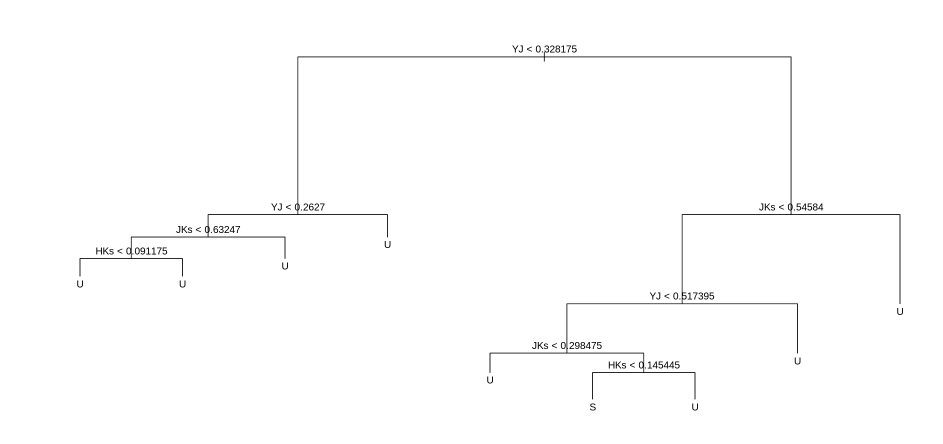
\includegraphics[width=0.7\linewidth]{Figuras/tree.png}
    \caption{Árvore de classificação para a amostra de asteroides.}
    \label{tree}
\end{figure}

\begin{figure}[h]
    \centering
    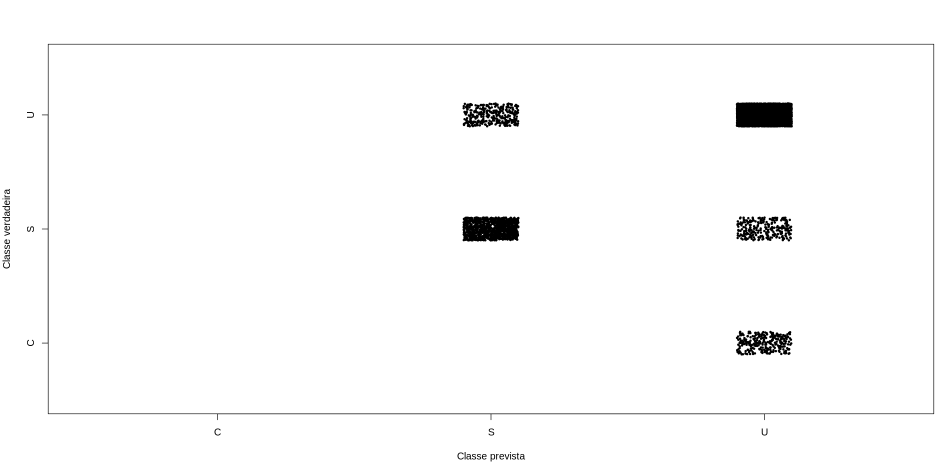
\includegraphics[width=0.8\linewidth]{Figuras/jitter.png}
    \caption{Gráfico jitter para o resultados da árvore de classificação aplicada na amostra de asteroides.}
    \label{jitter}
\end{figure}

\begin{lstlisting}
    # Data
    asteroid = read.table('/content/AsteroidClass.tsv', header=T, sep='|')
    asteroid = asteroid[complete.cases(asteroid),]

    # Packages
    install.packages('tree')
    library(tree)

    # Creating tree
    arv = tree(as.factor(Class) ~ HKs + JKs + YJ , data=asteroid)
    summary(arv)
    
    ### output ###
    
    Classification tree:
    tree(formula = as.factor(Class) ~ HKs + JKs + YJ, data = asteroid)
    Number of terminal nodes:  9 
    Residual mean deviance:  0.5786 = 4007 / 6926 
    Misclassification error rate: 0.1256 = 871 / 6935 
    
    # Plot
    plot(arv)
    text(arv)
    
    # Jitter plot
    pred = predict(arv, type = "class")
    asteroid$Class = as.factor(asteroid$Class)
    
    plot(jitter(as.numeric(pred), factor=0.5),
         jitter(as.numeric(asteroid$Class), factor=0.5),
         pch=20, cex=0.6,
         xlab='Classe prevista', ylab='Classe verdadeira',
         xlim=c(0.5, 3.5),
         ylim=c(0.5, 3.5),
         axes=FALSE)
    
    axis(1, at=1:3, labels=levels(asteroid$Class))
    axis(2, at=1:3, labels=levels(asteroid$Class))
    box()
\end{lstlisting}
